\section{Pianificazione} \label{sec:pianificazione}

Le due scadenze previste, la RTB e la PB, verranno suddivise in Sprint. 

\noindent
Ogni Sprint è associato ad una milestone, così facendo si mantiene un sistema di riferimento temporale e una struttura che permette di monitorare il progresso nel corso del progetto.

\vspace{0.3cm}
\noindent
Durante ciascuno Sprint sarà settato un obiettivo primario, ma si includeranno anche altre attività presenti nel Backlog. Questo modello Sprint consente al team di concentrarsi su compiti specifici e, allo stesso tempo, offre la possibilità di adattare attività che emergono durante lo sviluppo, garantendo un approccio più agile e adatto al cambiamento.

\noindent
La RTB verrà suddivisa nei seguenti Sprint con i relativi obiettivi primari:
\begin{itemize}
    \item Sprint-1 (dal 13/11/2023 al 03/12/2023): Analisi preliminare;
    \item Sprint-2 (dal 04/12/2023 al 17/12/2023): Progettazione Technology Baseline;
    \item Sprint-3 (dal 18/12/2023 al 31/12/2023): PoC - server;
    \item Sprint-4 (dal 01/01/2024 al 07/01/2024): PoC - email.
\end{itemize}

\noindent
La PB verrà suddivisa nelle seguenti fasi:
    \begin{itemize}
    \item Sprint-5 (dal 29/01/2024 al 04/02/2024): Architettura;
    \item Sprint-6 (dal 05/02/2024 al 18/02/2024): Progettazione;
    \item Sprint-7 (dal 19/02/2024 al 03/03/2024): Codifica;
    \item Sprint-8 (dal 04/03/2024 al 17/03/2024): Stress test;
    \item Sprint-9 (dal 18/03/2024 al 24/03/2024): Revisione generale.
\end{itemize}

La seguente pianificazione non riporterà azioni ritenute ovvie come lo sviluppo dei verbali o la verifica dei documenti. Queste attività sono descritte dettagliatamente nelle Norme di Progetto sezione xxxxxxx. %TODO



\subsection{RTB}

    \subsubsection{Sprint-1} \label{sec:pianificazione-S1}
    \textbf{Durata}: 3 settimane, dal 13/11/2023 al 03/12/2023.
    
    \noindent
    \textbf{Ruoli coinvolti}: Responsabile, Amministratore, Analista, Verificatore.

    \vspace{0.3cm}
    \noindent
    Questo Sprint ha come obiettivo primario l'analisi preliminare, con lo scopo di dare una base documentale solida al gruppo e individuare i requisiti del progetto.
    
    \vspace{0.3cm}
    \noindent
    Questo è l'unico Sprint con una durata di 3 settimane. È stata fatta questa scelta pessimistica in fase di pianificazione per permettere al gruppo di riallinearsi in seguito ad una disorganizzazione iniziale, dettata dall'inesperienza (\hyperref[sec:RO1]{RO1}), avvenuta in seguito all'aggiudicazione degli appalti (avvenuta il 06/11/2023) e prima della creazione di un piano di mitigazione adeguato per tale rischio. Infatti, come risulta dal diagramma di Gantt, si nota un rallentamento iniziale delle attività durante il quale ci impegneremo per riorganizzarci e definire adeguati piani di mitigazione.


        \paragraph{Pianificazione}
        \begin{itemize}
            \item obiettivi: dare un primo incremento alla documentazione per stabilire le regole necessarie allo svolgimento del progetto in modo coordinato. Redigere quindi il processo di documentazione e cominciare quello di gestione organizzativa nelle Norme di Progetto. Impostare inoltre il Piano di Progetto, il Glossario e l'Analisi dei Requisiti con particolare attenzione ai Casi d'Uso. Verrà inoltre creato un sistema di automazione per il way of working della documentazione;
            \item potenziali rischi: 
            \begin{itemize}
                \item RO1 - inesperienza con i progetti (\ref{sec:RO1});
                \item RO4 - distribuzione disomogenea (\ref{sec:RO4});
            \end{itemize}
            \item compiti:
                \begin{itemize}
                    \item Norme di progetto: l'Amministratore si occupa di redigere la parte di documentazione e gestione organizzativa;
                    \item Analisi dei Requisiti: gli Analisti si occupano di identificare e redigere i Casi d'Uso;
                    \item Piano di Progetto: il Responsabile si occupa di redigere la pianificazione dello Sprint-1, l'analisi dei rischi e il calendario di massima;
                    \item Glossario: l'Amministratore si occupano di redigere una prima versione del Glossario;
                    \item sistema di automazione: l'Amministratore si occuperà di implementare il sistema di automazione per il way of working della documentazione.
                \end{itemize}
        \end{itemize}
        
        \clearpage
        \paragraph{Gantt}
        
        \begin{figure}[H]
            \centering
            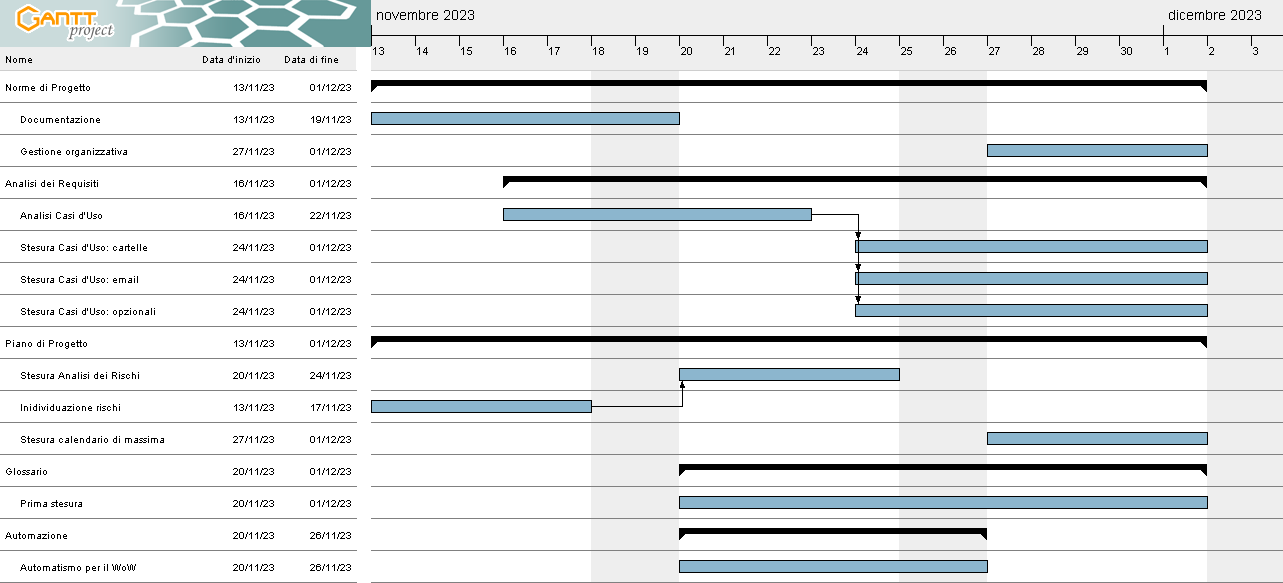
\includegraphics[scale=.44]{imgs/sprint1.png}
            \caption{grafico di Gantt relativo allo Sprint-1}
            \label{fig:gantt-sprint1}
        \end{figure}
        \clearpage
